\section{Secure Functionalities}
\label{sec:technique-in-depth}

\subsection{Secure device Discovery}
\label{subsec: Secure device Discovery}
 Device discovery serves two functions: 1) it is used in the context of discovering neighboring embedded systems to form routing paths, where existing mechanisms can be used and 2) for device on-boarding. During on-boarding, the Embedded system passes its device-level information (such as manufacturer-ID and model number) and application-level information (such as service type and data type) to the upstream devices. But, if the device is required to have a globally unique ICN ID, it can be provided one by the naming service.\par
  \begin{figure}[ht]
	\centering
	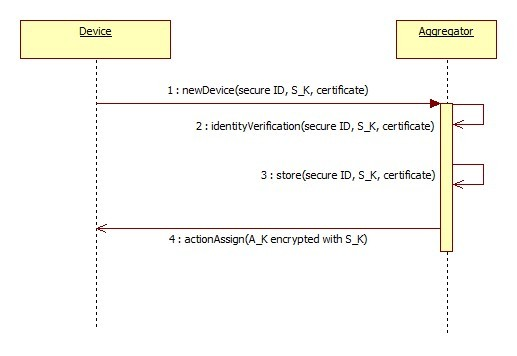
\includegraphics[width=\linewidth]{Figures/Secure-device-discovery-with-pre-load-secure-keys.png}
	\caption[]{Secure device Discovery with pre-load secure keys}
	\label{fig:Secure device Discovery with pre-load secure keys}
\end{figure}
 In the name-based ICN approaches where device identity is not needed, a device can publish within the name scope of the aggregator. In most IoT systems, devices interact with the aggregator for data or information processing or aggregation, hence there is no direct communication between devices under an aggregator. If in some set-up devices under the aggregator need to communicate with each other a scalable mechanism is to allow direct neighbors to communicate with each other while others communicate through the aggregator.\par
 \begin{figure}[ht]
	\centering
	\includegraphics[width=\linewidth]{Figures/Secure-device-discovery-without-key.png}
	\caption[]{Secure device Discovery}
	\label{fig:Secure device Discovery}
\end{figure}

 \begin{figure*}[ht]
	\centering
	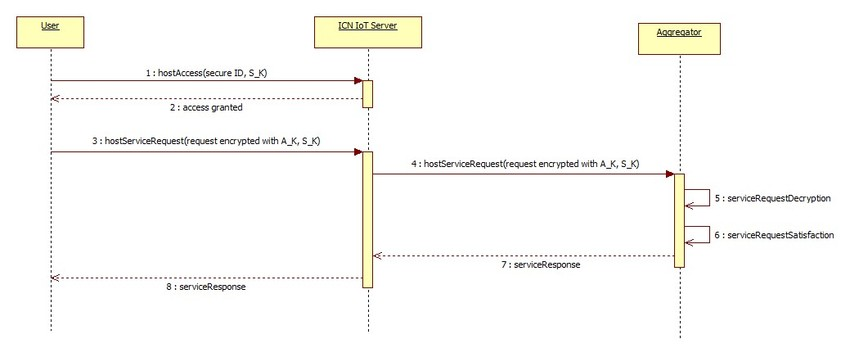
\includegraphics[width=\linewidth]{Figures/Secure-service-discovery.png}
	\caption[]{Secure service Discovery}
	\label{fig:Secure service Discovery}
\end{figure*}
 Based on our architecture model, we would discuss, what are the different functions of the elements of this ICN system that infer secure functionalities to out IoT devices. As discussed, the aggregator is the direct connection to other devices and we shall see its involvement for these functions.\par As and when a new IoT device is in the vicinity of the aggregator, it will pass on its device level information such as its manufacture ID or model number and its application level information such as its service type or data-type to the aggregator. The aggregator would then forward this information to the device that assigns unique names and returns this assignment back to the device. In doing so, it also stores this mapping of name and device for future communication.\par But how is this secure? To answer this question, we shall look at the UML diagram Fig. \ref{fig:Secure device Discovery with pre-load secure keys}, where device discovery takes place due to pre-loaded secure keys. In this scenario, the embedded system is programmed by its owner with a secure ID, a public/private key pair and certificate. This information is then transmitted to the aggregator. The aggregator implements the access control mechanism and verifies the device identity and it assigns it according to the access permission policies. In order to achieve integrity and confidentiality, the device does not send its private key, but a signature derived from its private key. This is sent to the aggregator along with its certificate. The aggregator returns an action key to this device after verification. This action key is encrypted by the signature received from the device. This action key is henceforth used by the device for secure communication of future data transmissions. \par
 
Secure device discovery can also occur when the embedded system is not programmed by the owner but by the manufacturer itself. In this case, the manufacture ID , a public private key pair and its certificate will already be available on the device at the time of purchase. This method is less robust but by implementing a web-of-trust model or by ensuring that the same manufacture has provided the devices, we can trust the authenticity of the devices. This however makes us dependent on the manufacture and hence an implementation of three factor authentication by user after obtaining the device could be a round about. The same principle works as above. This can be inferred through the UML diagram Fig. \ref{fig:Secure device Discovery}.\par



First, the device sends its secure Manufacture ID to inform that it is in the vicinity. The aggregator responds with sending it its signature key and certificate. Here we must implement the three way authentication. The device will now send the secure ID encrypted with the signature which will be verified by the aggregator. In response to a positive verification, the action key will be returned to the device. This action key would be used in future secure communication between the device and the aggregator.
 \begin{figure*}[ht]
	\centering
	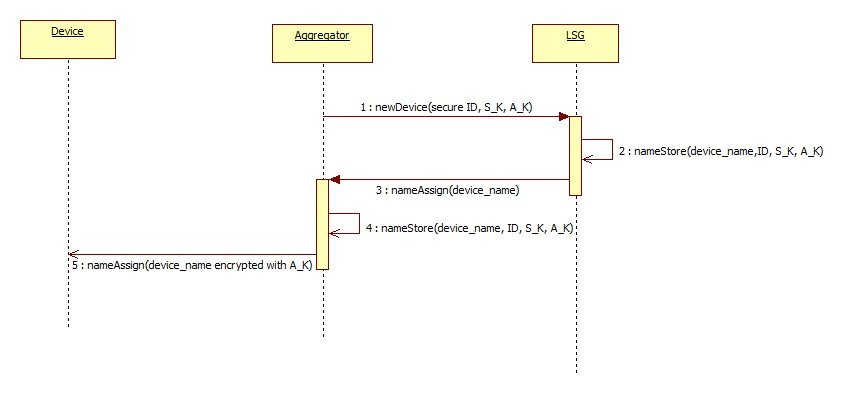
\includegraphics[width=\linewidth]{Figures/Secure-naming-service.jpg}
	\caption[]{Secure naming service}
	\label{fig:Secure naming service}
\end{figure*}

\subsection{Secure service Discovery}
As important as it is to secure the system for illegitimate devices, it is equally important that any illegitimate user does not access services that were intended to be hidden to this user. In order to distinguish which embedded device or user is allowed to access which services ,certain access control policies are implemented through names assigned to these devices. Let us look at the UML diagram for secure service discovery in Fig. \ref{fig:Secure service Discovery}.\par

Here, we can see the actions taken by a legitimate user that requests a certain service from the network. First, the user/device  would ask the ICN-IoT Server permission to access the service. If the user is allowed to access this service then, the server permits an access grant on this device. The device now sends out a service request to the server in an encrypted manner. The encryption takes place with the action key that was earlier alloted to it by the aggregator. To maintain confidentiality and integrity this encrypted message is signed with the signature key. The server forwards this encrypted request to the respective aggregator that is responsible for this service. There, the aggregator will first decrypt the request and if it can, it will satisfy the request and send it on to the server. The server will simply forward this response to the requesting device. This works brilliantly in a distributed IoT system but as it is obvious from this example. We require a server that implements the access control mechanisms. 

\par
\subsection{Secure naming service}
\label{subsec: Secure naming service}
If a device needs a global unique name/ID, but does not have one, it may request the naming service to obtain one after it is authenticated. Alternatively, the IoT domain (LSG or aggregator) may determine ID (name) for an authenticated device, which is required based on the access control policy. The proposed naming process works as follows. After a device has been authenticated, it may request an ID from the naming service (or the aggregator, if it can give the device a locally unique name). It sends a ID request (IDReq) to the naming service or aggregator. If the aggregator can accept request to give a unique name to the device, it will do that.\par

\par
In Fig. \ref{fig:Secure naming service}, we see the UML diagram for naming service. As and when a new device is detected, the aggregator forwards its secure ID, signature ID and action key to the Local service gateway(LSG), which is responsible for name allocation. The LSG stores these values and finds a suitable ICN name based on its access policies for this device. Along with this name it also generates a certificate that binds the name to its signature key. This certificate infers authenticity to the device. Once a name is generated it is sent to the aggregator along with its certificate, which in turn is stored at the aggregator. The name assigned by the LSG is encrypted with the action key and forwarded to the device.

\subsection{User registration}
\label{subsec:User registration}
For a distributed system with heterogeneous embedded IoT devices, the ICN-IoT Server provides the signature key and action key required by the device for all of their functionalities. A user must register itself in order to be discovered by the aggregator to avail any services of the network. 
In order to do so, the user sends relevant information about himself or herself to the ICN-IoT Server as per the requirements of this application. But how can we be sure that the details entered belong to you? i.e how do we authenticate you, this will be discussed in the later section \ref{sec:discussion}  discussion of this report. \par
In Fig. \ref{fig:User registration}, we see the UML diagram for user registration. Here the user sends his information to the ICN-IoT server, the server verifies this registration and returns three values back to the user: identifier, signature key and a temporary password. The user is then invoked to change his received password. Once this password has been set, the server sends the user the action key encrypted along with its signature key.
Hence, upon successful registration the IoT server securely transmits an identifier, a user signature key SK (to be used to sign messages), a user encryption key action key AK (to communicate data confidentially), and an access password to the user in an encrypted message, which is changed by the user at reception.
 \begin{figure}[ht]
	\centering
	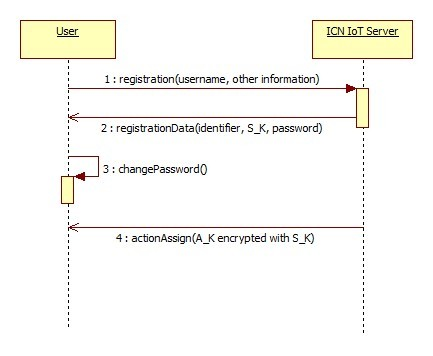
\includegraphics[width=\linewidth]{Figures/User-registration-secure-subscribe.png}
	\caption[]{User registration}
	\label{fig:User registration}
\end{figure}
\par
\subsection{Secure content delivery}
So far we have discussed about how a user is securely registered by the system, how it is securely discovered by the network, how a new device is named according to its access policies and how a legitimate device w.r.t its name finds a service in the network. Now we come to the last important security question: How do we secure the content that is delivered to the device from the service? \par 
To answer this question we relay the entire scenario again. After a new device has been registered and discovered by the network, it sends its ICN name, ID encrypted by signature key and service request encrypted by action key to the aggregator. The aggregator relates the ICN name (obtained at ICN naming \ref{subsec: Secure naming service}) to map the devices action key (obtained at device discovery \ref{subsec: Secure device Discovery}) and decrypts the request and to verify that it is the legitimate device it decrypts the ID with the stored signature key. If the ID matches the stored device ID then the device is authenticated. Hence the request is forwarded to the server that fulfills the request and responds with the service content. \par
Now depending on the application, the content delivered from the server is secured with an encryption with the action key. The device must then apply decryption to read the contents and use it for its application however if this device is a light weight embedded system then it may choose not to have this encryption and use the delivered plain text content. However this is not recommended. There are other methods to increase the speed at which the delivery is made and that is through caching of data close to the legitimate devices. Another way is to use group multi-cast secure keys to relay the same information to all legitimate devices of the same group. This increases the performance of the whole system.

Fig. \ref{fig:Secure content delivery}.
 \begin{figure}[ht]
	\centering
	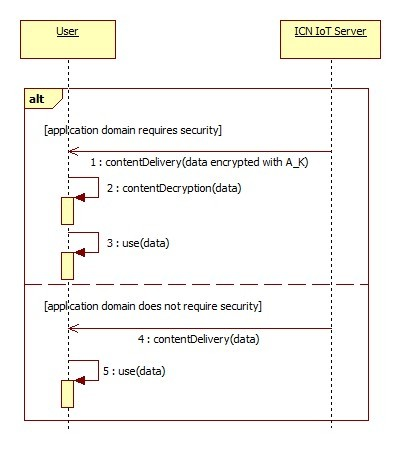
\includegraphics[width=\linewidth]{Figures/Secure-content-delivery-user.png}
	\caption[]{Secure content delivery}
	\label{fig:Secure content delivery}
\end{figure}
\par
